% This file contains the content for a main section
\numberedformat
%% Modify below this line %%
\chapter{Top-level schematic for the ACES user experience}

\autoref{fig:schematic} is the overview diagram for the ACES 1.0 user experience. This is not intended to replace the earlier conceptual block diagrams. However, it must be realized that those diagrams were intended primarily for an audience of color scientists and post-production engineers rather than the much wider audience of end-users being targeted for the 1.0 release.

Notice that acronyms have been eliminated. The names have been made shorter and more intuitive (definitions are provided in \autoref{sec:terminology}).

Please note that the Output Transform is the combination of the RRT with an ODT. A diagram showing the user-centric terms in relation to the engineering-centric block-diagram is provided in Appendix \ref{appendixA}, along with definitions of the engineering terms.

\begin{figure}[htbp]
\begin{center}
    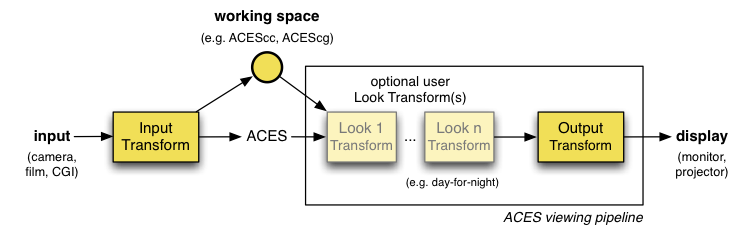
\includegraphics[width=\textwidth]{topLevelSchematic.png}
\caption{The top-level schematic for the ACES user experience}
\label{fig:schematic}
\end{center}
\end{figure}
